
\documentclass[10pt,a4paper]{article}
\usepackage[utf8]{inputenc}
\usepackage[spanish]{babel}
\usepackage{amsmath}
\usepackage{amsfonts}
\usepackage{amssymb}
\usepackage{makeidx}
\usepackage{graphicx}
\usepackage{cite} % para contraer referencias
\usepackage{fourier}
\usepackage{xcolor}
\usepackage{hyperref}
 \usepackage{float}
\usepackage[bottom]{footmisc}
\usepackage[left=2cm,right=2cm,top=2cm,bottom=2cm]{geometry}
\title{Plan - sesión 5}


\author{\textbf{Victor M. Santos}\thanks{victorhugo\_m09@hotmail.com}, \textbf{M.Tarazona-Alvarado}\thanks{miguelta281@gmail.com}, \textbf{J. Pisco-Guabave} \thanks{jhojavi@gmail.com}. \\ Grupo Halley , \\ Universidad Industrial de Santander, Bucaramanga, Colombia.}


\date{ }


\begin{document}

\maketitle
\tableofcontents
\section{Objetivo}
Reconocer las diferentes propiedades de la luz en aplicaciones propias de la astronomía.

\section{Contenido}
\begin{itemize}
\item Propiedades de la luz
\begin{itemize}
\item Reflexión
\item Refracción
\item Dispersión
\item Difracción
\end{itemize}
\end{itemize}


\section{Recursos}
\begin{itemize}
 \item Salón con capacidad para 20 personas
 \item Proyector
 \item Computador
 \item Marcadores
 \item Tablero
 \item Espacio al aire libre (amplio)
\end{itemize}

\section{Marco conceptual}
\subsection{Propiedades de la luz}
La luz es la fracción del espectro electromagnético que el ojo humano puede percibir, esta región se encuentra entre los 400 y 700 nm. La luz, como el resto de radiación del espectro electromagnético, posee algunas propiedades que la caracterizan, entre ellas se encuentran la reflexión, refracción, dispersión y difracción. Estas características son las más conocidas y las de nuestro interés, aunque no son las únicas.
\begin{figure}[H]
\centering
%\raggedright
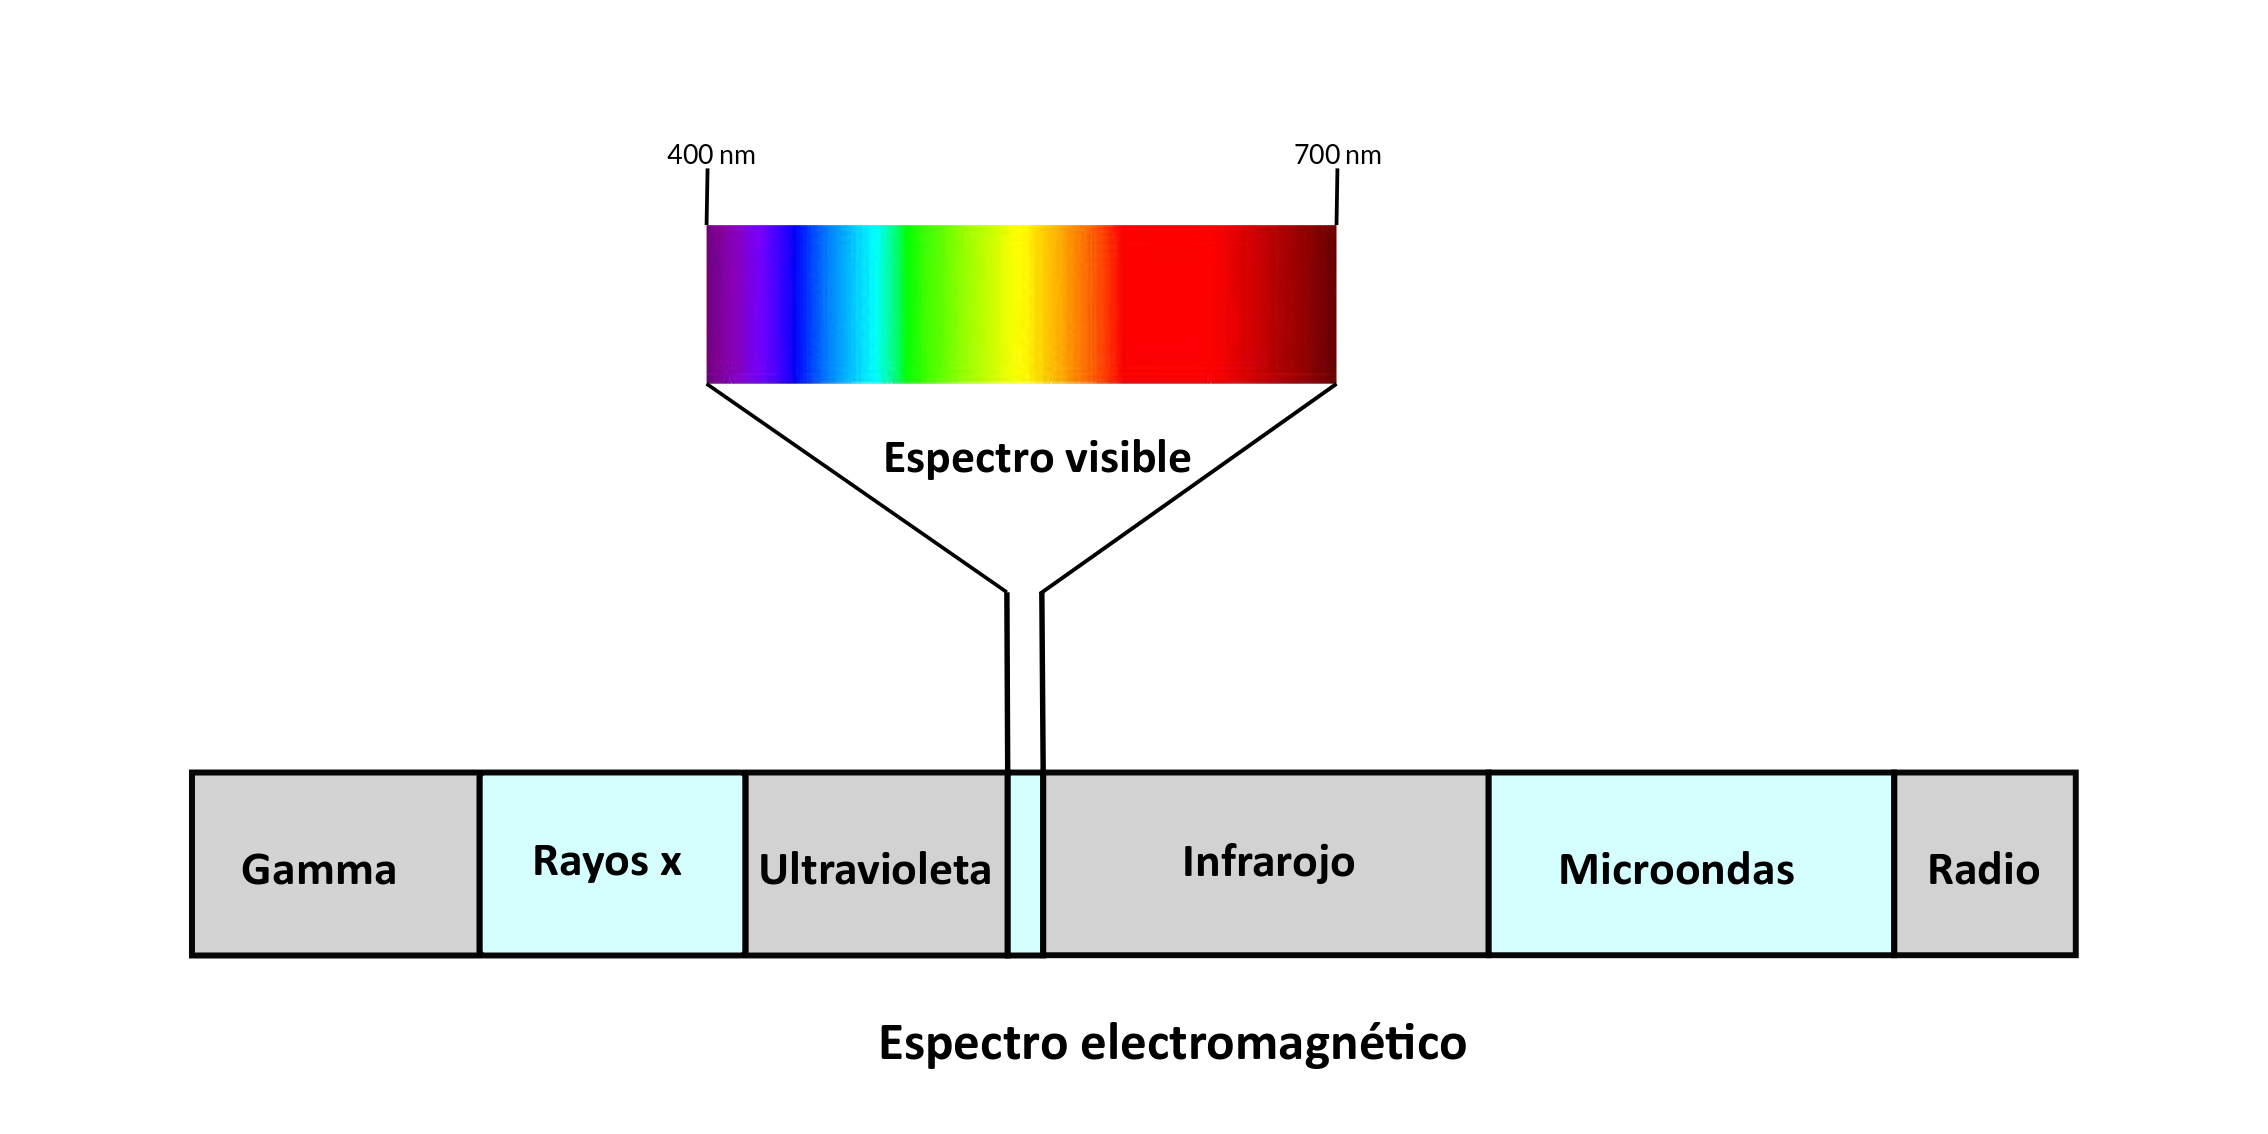
\includegraphics[scale=0.18]{Imagenes/Espectro_01}
\end{figure}


\subsubsection{Reflexión}
La reflexión es el cambio en la dirección que experimenta un rayo de luz cuando incide sobre una superficie opaca. Las superficies pulimentadas suelen presentar este fenómeno según la ley de reflexión, esto es que el ángulo de incidencia del rayo de luz y el ángulo de reflexión son equivalentes.
\begin{figure}[H]
\centering
%\raggedright
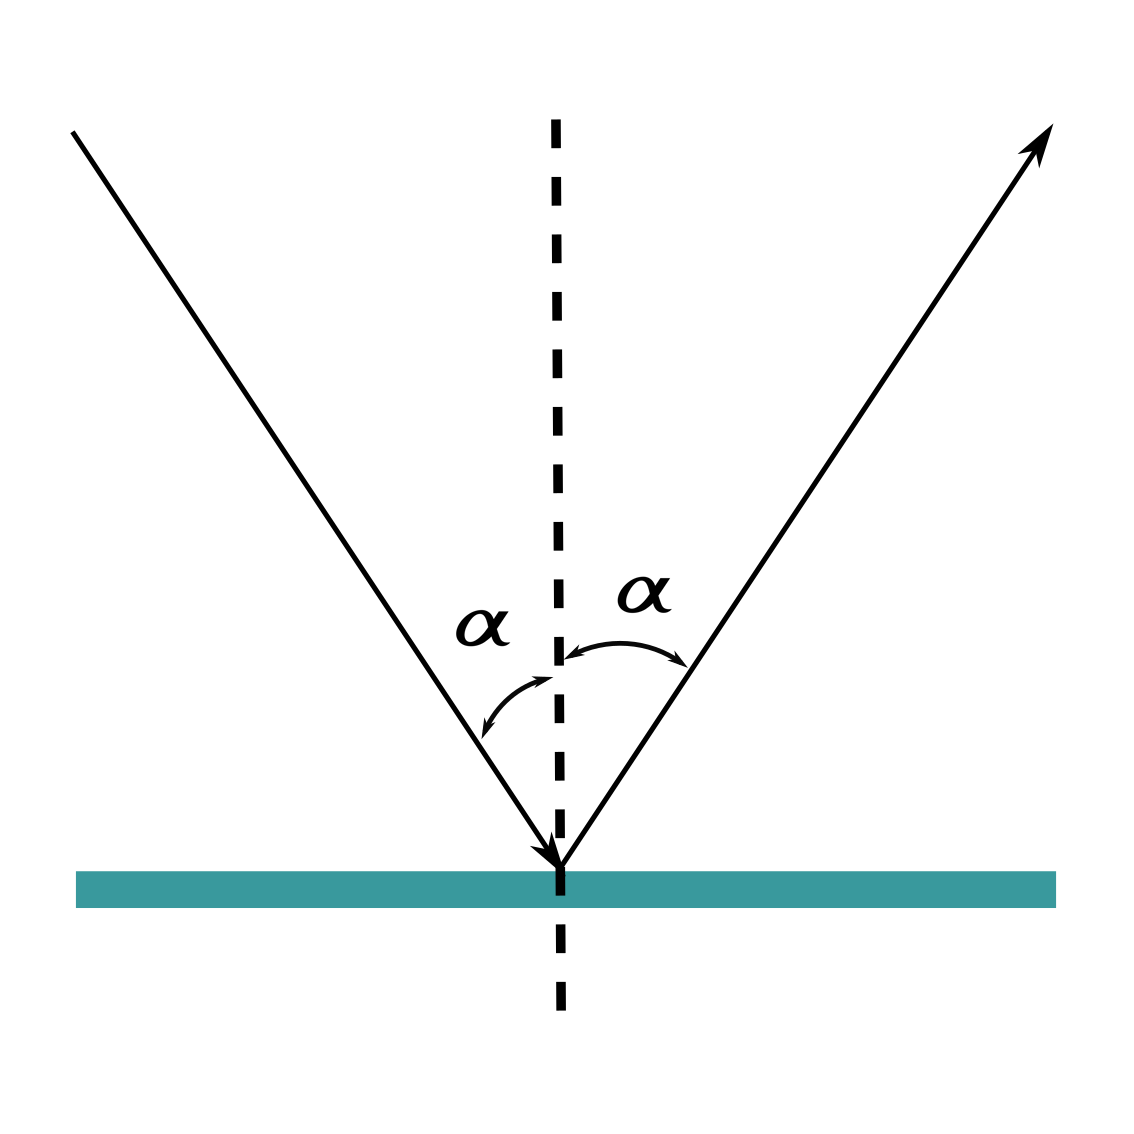
\includegraphics[scale=0.18]{Imagenes/Reflexion_01}
\end{figure}

\subsubsection{Refracción}
La refracción es el cambio de velocidad que experimenta una onda de luz al pasar de un medio a otro con distinto índice refractivo. Este cambio de velocidad que experimenta el rayo de luz causa el cambio en la dirección del mismo.
\begin{figure}[H]
\centering
%\raggedright
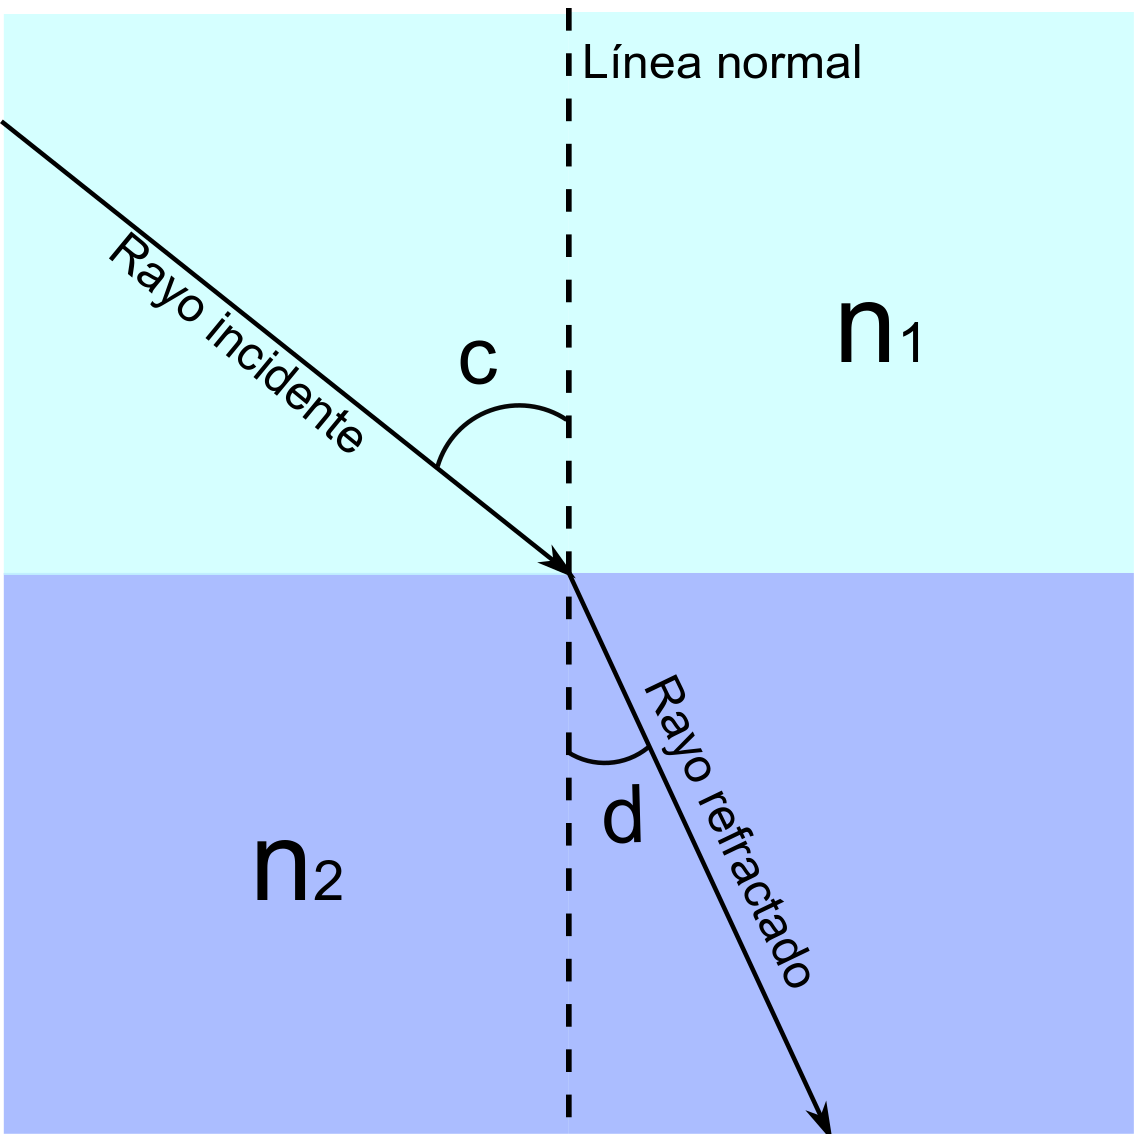
\includegraphics[scale=0.2]{Imagenes/Refraccion_01}
\end{figure}

\subsubsection{Dispersión}
La dispersión es otro fenómeno asociado a las ondas. En este caso, cuando la luz blanca incide en un prisma, se separa en ondas de distintas frecuencias.  También presenta una estrecha relación con la refracción, ya que distintas radiaciones monocromáticas (que corresponden a un solo color) son más desviadas por la refracción cuanto menor es su longitud de onda. Es decir, la luz azul es más desviada que la luz roja. 
\begin{figure}[H]
\centering
%\raggedright
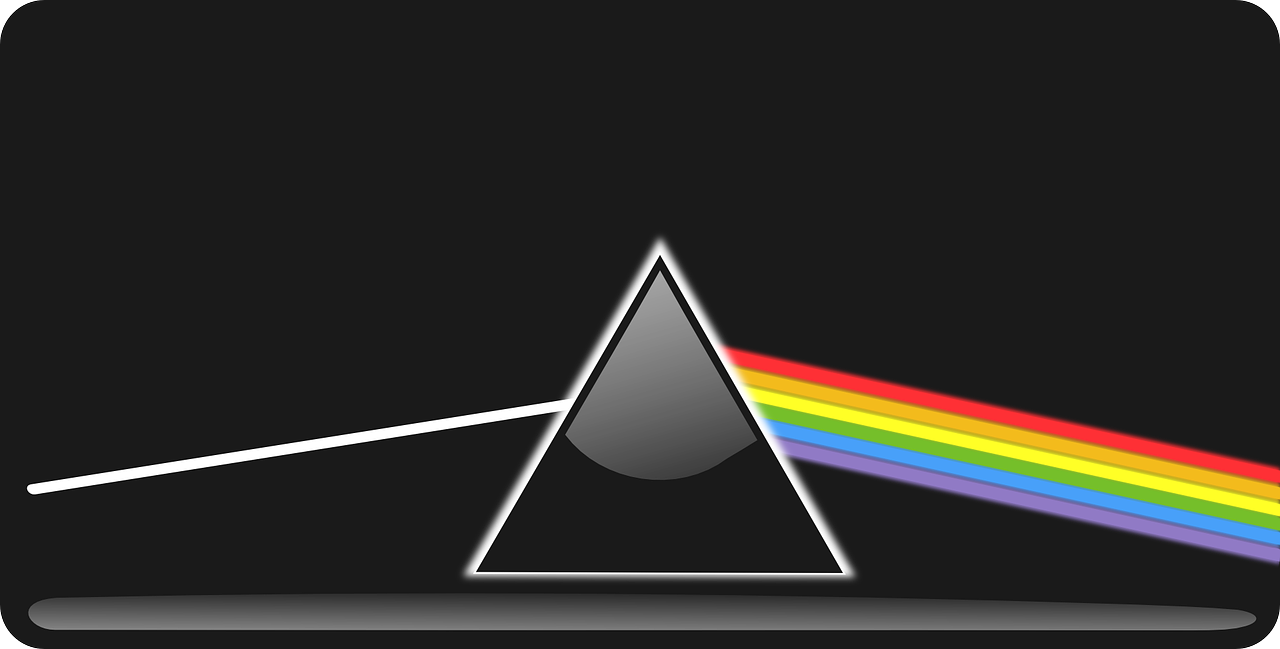
\includegraphics[scale=0.18]{Imagenes/Dispersion_01}
\end{figure}

\subsubsection{Difracción}
La difracción es un fenómeno característico de las ondas que se basa en la desviación de estas al encontrar un obstáculo o al atravesar una rendija.
\begin{figure}[H]
\centering
%\raggedright
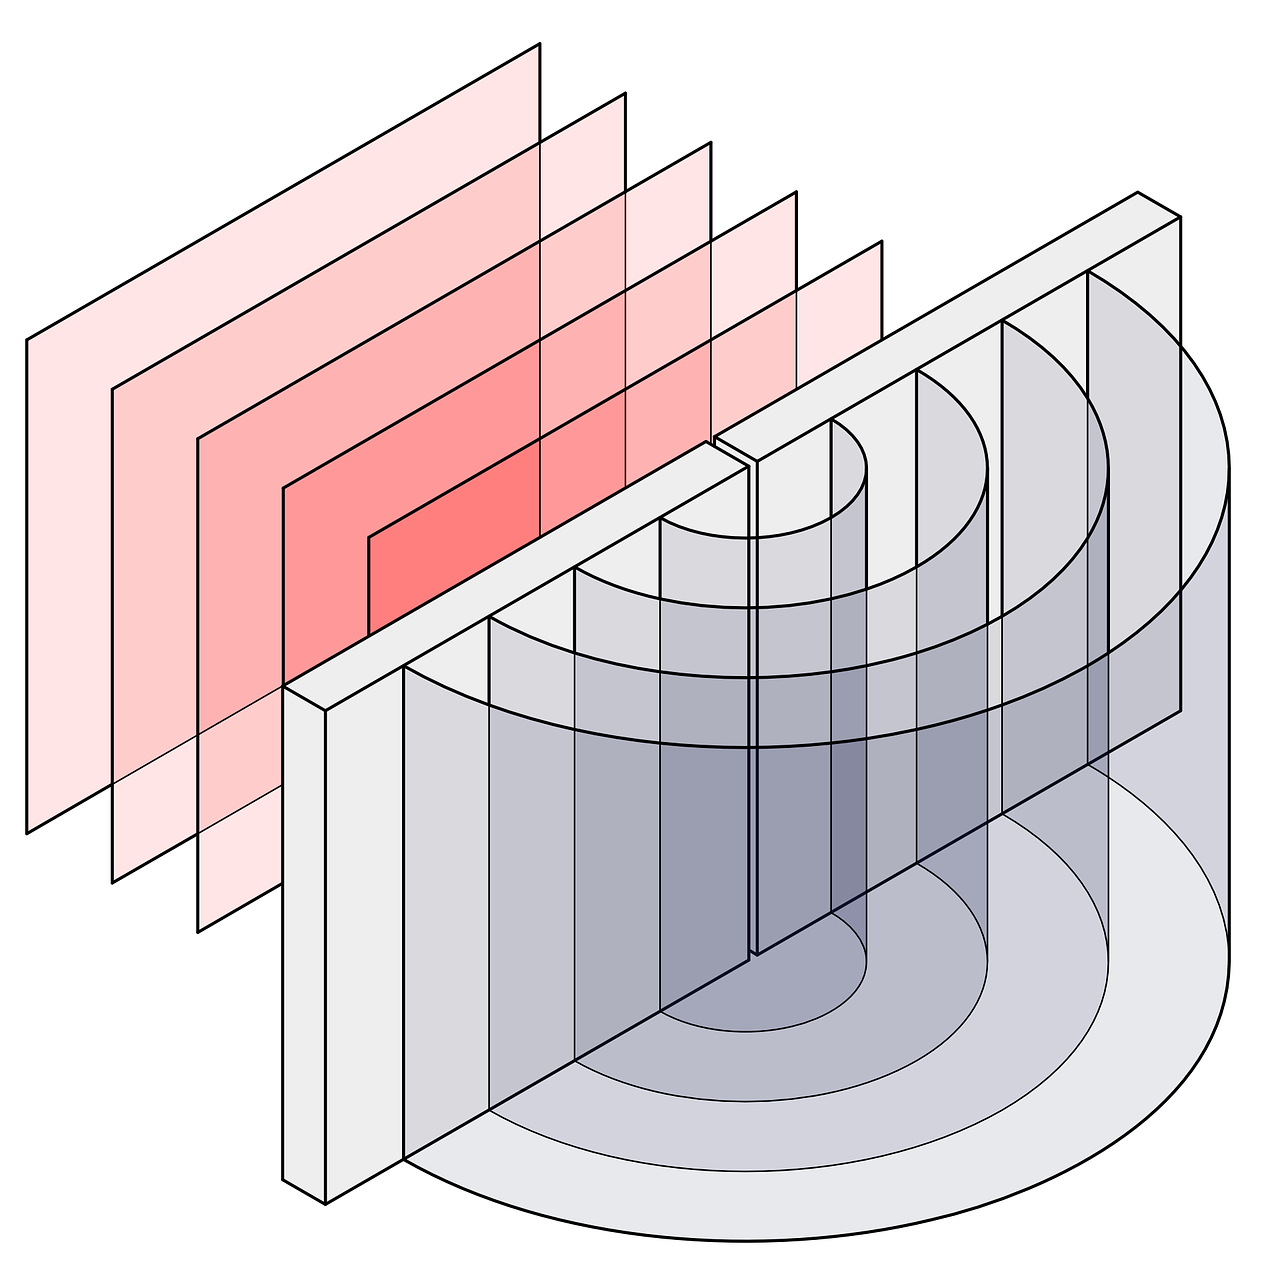
\includegraphics[scale=0.18]{Imagenes/Difraccion_01}
\end{figure}

\section{Planeación de la sesión}
\begin{table}[H]
\begin{tabular}{|l|l|l|l|}
\hline
\textbf{Etapa}      & \textbf{Tiempo} & \textbf{Actividad}      & \textbf{Recursos}   \\ \hline
\textbf{Inicio}     & 20 minutos      & S05AI01      & \begin{tabular}[c]{@{}l@{}}- Computador \\ - Proyector  \end{tabular} \\ \hline
\textbf{Desarrollo} &   60 minutos  &  \begin{tabular}[c]{@{}l@{}}S05AD01  \\ S05AD02 \\ S05AD03 \\ S05AD04    \end{tabular}                                                                                       & \begin{tabular}[c]{@{}l@{}}- Prisma \\ - Globos \\ - Lupas \\ - Linterna (luz blanca) - Sextante \\ Cartulina (1/8)  \\ \end{tabular} \\ \hline
\textbf{Cierre}     &   40 minutos              &  S05AC01                                                                                    & \begin{tabular}[c]{@{}l@{}} - Tubo \\ - CD \\ - Cinta (negra) \\ - Cartulina \end{tabular} \\ \hline
\end{tabular}
\end{table}

Para el desarrollo de esta sesión se usará la presentación en la etapa de inicio y la de desarrollo. Cada lámina ejemplifica uno de los fenómenos más importantes.

\subsection{S05AI01}
Al inicio de esta sesión se mostrará la imagen asociada al fenómeno de refracción que está en la presentación. A continuación el tutor plantea una pregunta problema abstraída de la imagen, ¿por qué vemos que cambia el tamaño del limón cuando está detrás del vaso de agua?. Será que el limón cambia de tamaño? Los estudiantes deberán desarrollar teorías que expliquen el fenómeno mientras el tutor sigue cuestionando las explicaciones al fenómeno. Esta actividad pretende crear debate para acercarse a la explicación científicamente aceptada de este fenómeno y de otros que, de igual forma, afectan a las ondas electromagnéticas.

\subsection{S05AD01 (refracción)}
En esta actividad se usarán un globo de color negro, uno blanco, uno rojo, uno azul y uno verde. Para este experimento se usará la luz solar concentrada usando una lupa. Inicialmente, se inflarán todos los globos hasta que alcancen un tamaño similar. A continuación, se incide la luz blanca concentrada sobre cada uno de los globos en orden, tomando el tiempo que demora en explotar cada uno. Con este experimento se evidencian dos fenómenos importantes, por un lado la refracción de la luz al pasar por la lupa y, por otro lado, la absorción de energía que caracteriza a cada objeto (entre más energía absorbe el globo, más rápido explota).

\subsection{S05AD02 (Reflexión )}
La práctica para esta propiedad está ligada a un instrumento conocido como sextante. Este instrumento usa la reflexión para determinar la altura de los astros en la bóveda celeste.
%Reflexión 
\subsection{S05AD03 (dispersión)}
Se hace pasar luz blanca a través de un prisma. Como consecuencia el prisma separará las diferentes longitudes de onda que componen la luz blanca, haciendo evidente el fenómeno a estudiar. 
%dispersión 
\subsection{S05AD04 (Difracción)}
Se hace uso de una linterna. La luz que emite la linterna atraviesa parte de la misma, pasando por un agujero (por donde sale la luz de la linterna). Luego de pasar el agujero (salir de la linterna), la luz se extiende siguiendo el comportamiento de una onda.
%Difracción

\subsection{S05AC01}
En esta actividad se construye un espectroscopio casero. Este espectroscopio se vale de las propiedades de la luz para evidenciar el espectro de emisión de una fuente de luz, dispersando la luz y mostrando los diferentes colores que la componen. Este espectroscopio es construido individualmente por cada estudiante y será de propiedad de cada uno de ellos.

\begin{figure}[H]
\centering
%\raggedright
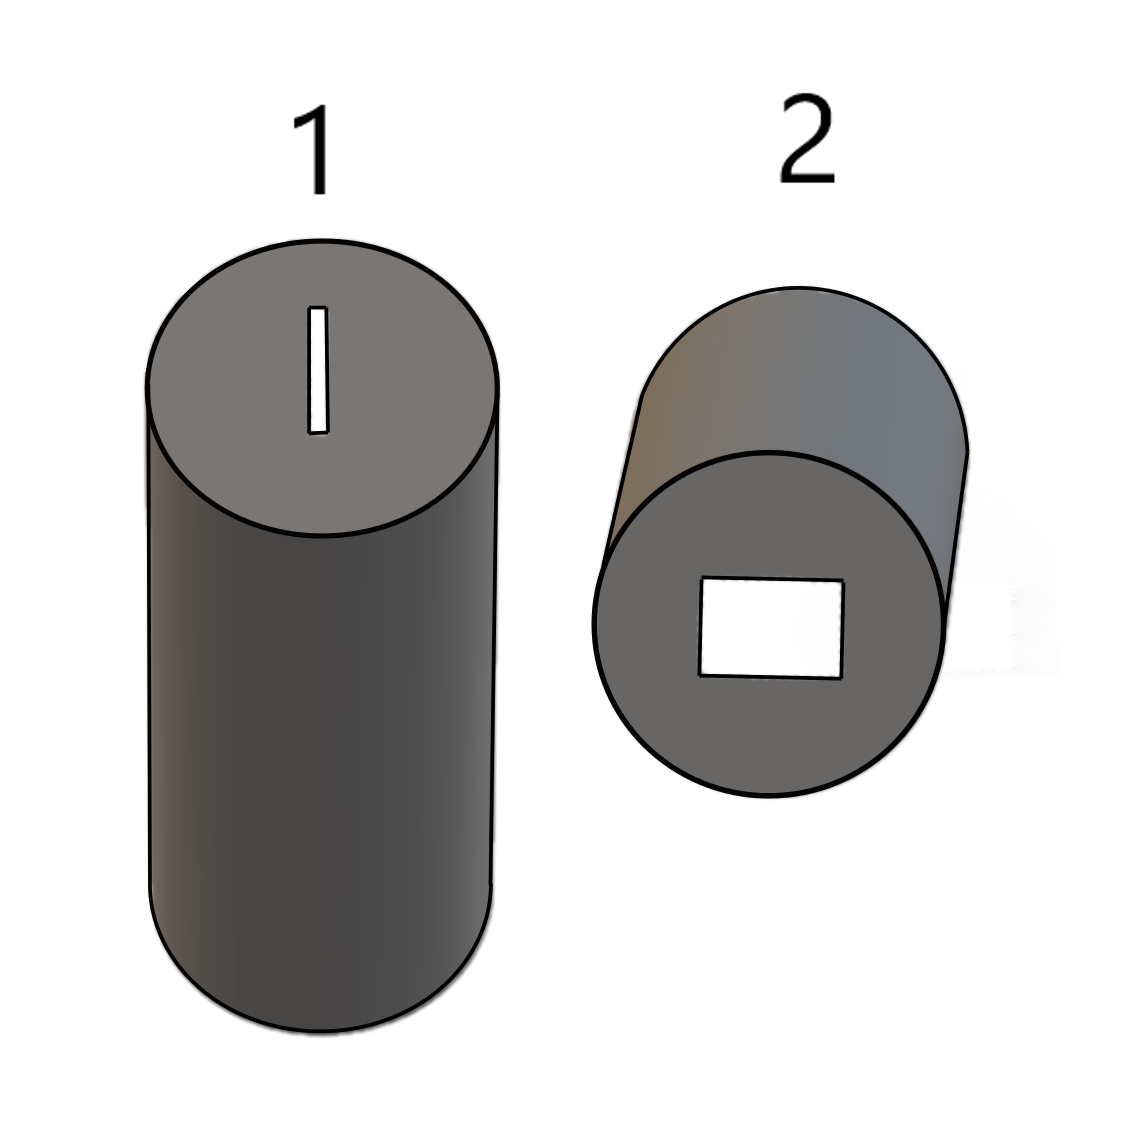
\includegraphics[scale=0.15]{Imagenes/actividad_cierre_01}
\end{figure}

\end{document}